%!TEX root = ../main.tex

\chapter{MPAI} \label{chp:mpai}
Come evoluzione del rinomato \ac{MPEG}, nel luglio 2020 nasce \ac{MPAI}\footnote{\url{https://mpai.community}}.

\ac{MPAI} è un'organizzazione non profit che, ancora guidata da Leonardo Chiariglione, ha come obiettivo la promozione dell'uso efficiente dei dati\footnote{Per dati \ac{MPAI} intende, per esempio, dati mediatici, manifatturieri, automobilistici, sanitari e generici. \cite{mpaiMPAICommunity}.} tramite lo sviluppo di specifiche tecniche per la codifica di qualunque tipo di dato facendo uso dell'intelligenza artificiale e la semplificazione dell'utilizzo di tali codifiche imponendo ai detentori di proprietà intellettuale di stabilire delle licenze per framework (\acs{AIF}), invece di dover essere legati ai brevetti e creare delle \textit{patent pool} \cite{mpaiMPAICommunity}. Sostanzialmente l'organizzazione si pone come missione quella di porre ordine nel mondo delle codifiche utilizzanti l'IA e di farlo semplificando il metodo di accesso alle proprie tecnologie rispetto ad \ac{MPEG}.
\ac{MPAI} opera attraverso la collaborazione delle varie parti interessate, tra cui l'università di Padova tramite il suo spin-off \href{www.audioinnova.com}{Audio Innova}.

In questi tempi l'utilizzo dell'intelligenza artificiale sta crescendo in maniera esponenziale e si sta avvicinando all'utente comune tramite la miriade di piattaforme online che sono nate, un esempio è \href{https://chat.openai.com}{ChatGPT} che ha raggiunto quota 100 milioni di utenti attivi in soli 2 mesi, raggiungendo il primato di applicazione ad uso privato con la crescita più veloce della storia.\footnote{\url{https://www.reuters.com/technology/chatgpt-sets-record-fastest-growing-user-base-analyst-note-2023-02-01/}} Nonostante il suo, come visto, uso spropositato l'IA è di fatto una tecnologia difficilmente comprensibile dalle masse; ciò porta l'utente a non capire che il \textit{chatbot} con cui sta interagendo, non replichi utilizzando un principio di causalità, ma piuttosto segua dei pattern linguistici i quali non sempre portano a risposte corrette, nonostante l'autorevolezza col quale l'IA sembri scrivere.

Il comitato di \ac{MPAI} si impegna ad affrontare col coinvolgimento di esperti esterni gli emergenti quesiti etici, i quali sono molto rilevanti a causa del rapido e soltanto recente sviluppo dell'IA.

Il progetto comprende diverse aree d'effetto tra cui il dialogo uomo-macchina, l'esperienza audio, la compressione video, l'esperienza di gioco online, la creazione di esperienze collaborative nel metaverso, la codifica di dati sanitari, i veicoli a guida autonoma e molti altri e la lista è in continua espansione.\footnote{Tutti i vari progetti sono visualizzabili sul \href{https://mpai.community/standards/}{sito di \ac{MPAI} alla voce \textit{Standards}}.}


\section{MPAI-AIF, \acs{AIW} e \acsp{AIM}} \label{sec:aif-aiw-aim}
Ogni standard \ac{MPAI} è un \ac{AIF} \cite{mpaiMPAIAIFMPAICommunity}: un ambiente che comprende diversi \ac{AIW}, ognuno che descrive un certo caso d'uso. I blocchi costituenti un workflow sono detti \acp{AIM} ed ogni modulo è definito dalla sintassi e dalla semantica delle proprie interfacce di input e output, l'implementazione (hardware o software che sia) non è specificata; i vari moduli svolgono delle specifiche attività e sono interconnessi a formare un AIW come si può vedere dalla figura \ref{fig:mpai-aif-architecture}.

\acs{AIF}, il modello fondante gli altri standard dell'organizzazione è stato adottato dall'\ac{IEEE} col nome \textit{IEEE 3301-2022} \cite{ieeeStandard3301-2022}.

\begin{figure}[h]
    \centering
    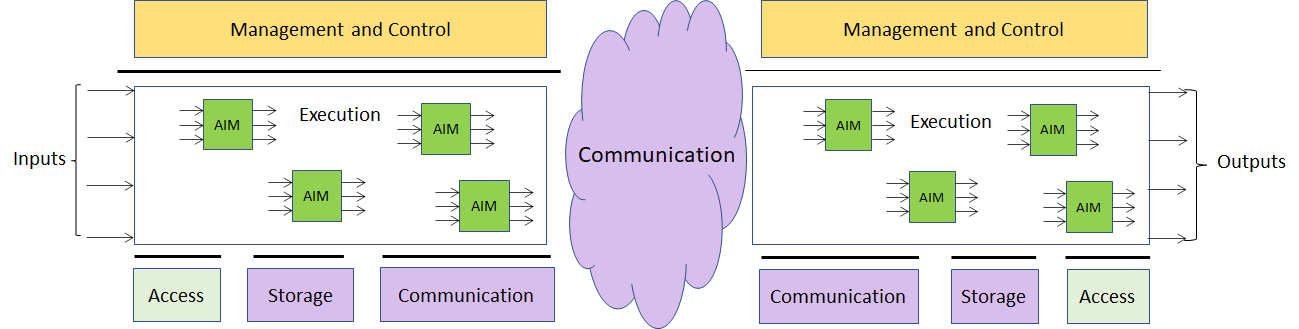
\includegraphics[width=\textwidth]{mpai-aif-architecture.png}
    \caption{Architettura di \acs{AIF} \cite{leonardoBlogNewWayDevelop2020}}
    \label{fig:mpai-aif-architecture}
\end{figure}


\section{Struttura di uno standard MPAI} \label{sec:standard-mpai} % e come implementarlo
Lo sviluppo di uno standard MPAI segue le fasi mostrate in figura \ref{fig:mpai-standard-stages}.    % TODO scrivere di più?

\begin{figure}[h]
    \centering
    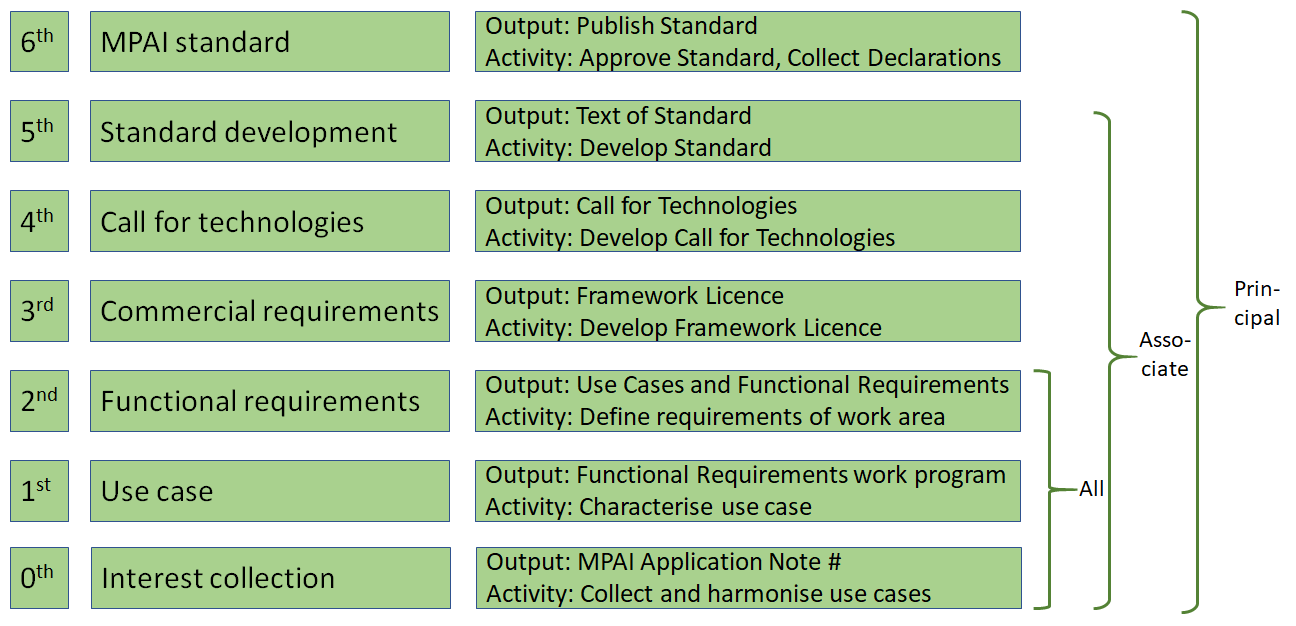
\includegraphics[width=\textwidth]{mpai-standard-stages.png}
    \caption{Le fasi dello sviluppo di uno standard \acs{MPAI} \cite{leonardoBlogNewWayDevelop2020}}
    \label{fig:mpai-standard-stages}
\end{figure}

Uno standard \ac{MPAI} è composto da un insieme di 4 documenti con i relativi software e dataset \cite{mpaiStructureMPAIStandards}:
\begin{description}
    \item[Specifiche tecniche (\textit{Technical Specification})] Contiene le norme che un'implementazione conforme deve necessariamente seguire; solitamente è un insieme di casi d'uso. Per ogni caso d'uso viene specificato l'\ac{AIW} che lo implementa con le funzioni che esegue, la sintassi e la semantica dei suoi dati in input ed output; la topologia degli \acp{AIM} costituenti l'\ac{AIW} e, per ogni \ac{AIM}, la loro funzione e la sintassi e la semantica dei loro input ed output. 
    \item[Software di riferimento (\textit{Reference Software})] Contiene il codice sorgente dell'implementazione delle specifiche tecniche dell'\ac{AIF} e dei suoi \ac{AIW} esponendo le interfacce dei propri \acp{AIM}. Inoltre il software deve essere fornito di un metodo per l'uso, la sua documentazione necessaria\footnote{Una \ac{KB}} ed eventualmente dei dati di esempio.
    \item[Test di conformità (\textit{Conformance Testing})] Un insieme di vincoli relativi all'output generato da un dato input a cui un'implementazione deve sottostare per essere definita conforme. Questo documento viene trattato in maniera più approfondita al capitolo \ref{chp:conformancetesting}.
    \item[Valutazione delle prestazioni (\textit{Performance Assessment})] Definisce gli attributi di Affidabilità (rispetto dello standard), Robustezza (capacità di gestione di nuovi dati), Equità (IA unbiased\footnote{Un'intelligenza artificiale può essere \textit{biased}, ovvero può "avere pregiudizi"; nel caso ottimo sono molto limitati (IA unbiased) perchè portano ad assunzioni errate.}) e Replicabilità (della valutazione) che vengono utilizzati per attribuire un voto all'implementazione (eventualmente dipendente da un certo dominio di applicazione).
\end{description}

\begin{adjustbox}{width=\textwidth}
    \begin{tikzpicture}[
        state/.style={rectangle, draw=black, align=center, minimum size=5mm},
    ]
        %Nodes
        \node[state]  (TS)                    {Specifiche\\tecniche};
        \node[state]  (RS)    [right=of TS]   {Software\\di riferimento};
        \node[state]  (CT)    [right=of RS]   {Test\\di conformità};
        \node[state]  (PA)    [right=of CT]   {Valutazione\\delle prestazioni};
        
        %Lines
        \draw[->] (TS.east) -- (RS.west);
        \draw[->] (RS.east) -- (CT.west);
        \draw[->] (CT.east) -- (PA.west);
    \end{tikzpicture}
\end{adjustbox} % TODO decidere se inserire in una figure?


\section{MPAI-CAE} \label{sec:mpai-cae}
Tra i vari standard/framework, \ac{CAE} si occupa di utilizzare le informazioni sul tipo di esperienza audio vissuta dall'utente (intrattenimento, teleconferenza, restauro, ...) e 'informazione del contesto in cui si trova (a casa, in auto, in mobilità, in studio, ...) per agire sul contenuto dell'audio in input e fornire i risultati desiderati \cite{mpaiMPAICAE}.

Sono considerati 4 casi d'uso:
\begin{description}
    \item[\ac{EES}] Permette all'utente di scegliere un'emozione ed ottenere successivamente una traccia audio di parlato con la tonalità specifica tipica dell'espressività indicata.
    \item[\ac{ARP}] Permette di creare copie di audio digitalizzato, valido per una conservazione a lungo termine e per una riproduzione corretta della registrazione.
    \item[\ac{SRS}] Permette di ripristinare un segmento danneggiato di traccia audio contenente il parlato di un singolo oratore sintetizzando la voce della parte corrotta.
    \item[\ac{EAE}] Permette di migliorare la qualità sonora in un'audioconferenza utilizzando i segnali registrati da array di microfoni rimuovendo rumori di fondo e artefatti acustici.
\end{description}

\ac{CAE} è stato adottato dall'\ac{IEEE} come standard \textit{IEEE 3302-2022} \cite{ieeeStandard3302-2022}.

Nel documento \citetitle{ieeeStandard3302-2022} si possono trovare tutte le informazioni sullo standard.


\subsection{MPAI-CAE-ARP} \label{ssec:mpai-cae-arp} % è l'implementazione del metodo del CSC, cos'è un codec, cosa fa, quali sono i suoi moduli
La procedura di digitalizzazione del \ac{CSC} introdotta nella sezione \ref{sec:csc-digitalizzazione} è stata proposta ad \ac{MPAI} ed è stata riconosciuta per la sua efficacia ed affidabilità, perciò è stata adottata come use case di \ac{CAE} col nome \acf{ARP}.\footnote{Le informazioni di questa sottosezione sono tratte da \cite{mpaiMPAIDataCoding}; maggiori informazioni nelle specifiche tecniche \cite{ieeeStandard3302-2022} e nella video presentazione del software di riferimento \cite{mpaistandardsMPAIPresentsContextbased2023}}

Il \ac{CSC}, con l'aiuto di vari collaboratori, ha prodotto anche un software di riferimento per \ac{ARP}, il quale non è altro che una codifica\footnote{Un codec (audio) è un software o un dispositivo che codifica o decodifica un segnale o uno stream di dati secondo una specifica convenzione.} audio lossless.

Nel 2023 Audio Innova è stata insignita del \textit{Cannes Neurons Award 2023 Palm d'Or} per il miglior progetto di utilizzo creativo di IA, \ac{ARP}, al World AI Cannes festival.\footnote{\url{https://mpai.community/2023/02/17/mpai-member-audio-innova-srl-received-the-cannes-neurons-award-2023-palm-dor/}}

Dati in input (vedi figura \ref{fig:arp-workflow}):
\begin{description}
    \item[Preservation Audio File] La copia digitalizzata dell'audio.
    \item[Preservation Audio-Visual File] Il file video prodotto dalla ripresa della testina di registrazione e del capstan (come in figura \ref{fig:tape-areas}).
\end{description}

Si ottengono in output (vedi figura \ref{fig:arp-workflow}):
\begin{description}
    \item[Access Copy Files] Il file audio restaurato, una lista delle modifiche effettuate, la lista delle irregolarità con relativa classificazione e le loro istantanee dal video.
    \item[Preservation Master Files] Il file audio di input, il file video con l'audio sostituito da quello registrato e sincronizzato, la lista delle irregolarità con relativa classificazione e le loro istantanee dal video.
\end{description}

\begin{figure}[H]
    \centering
    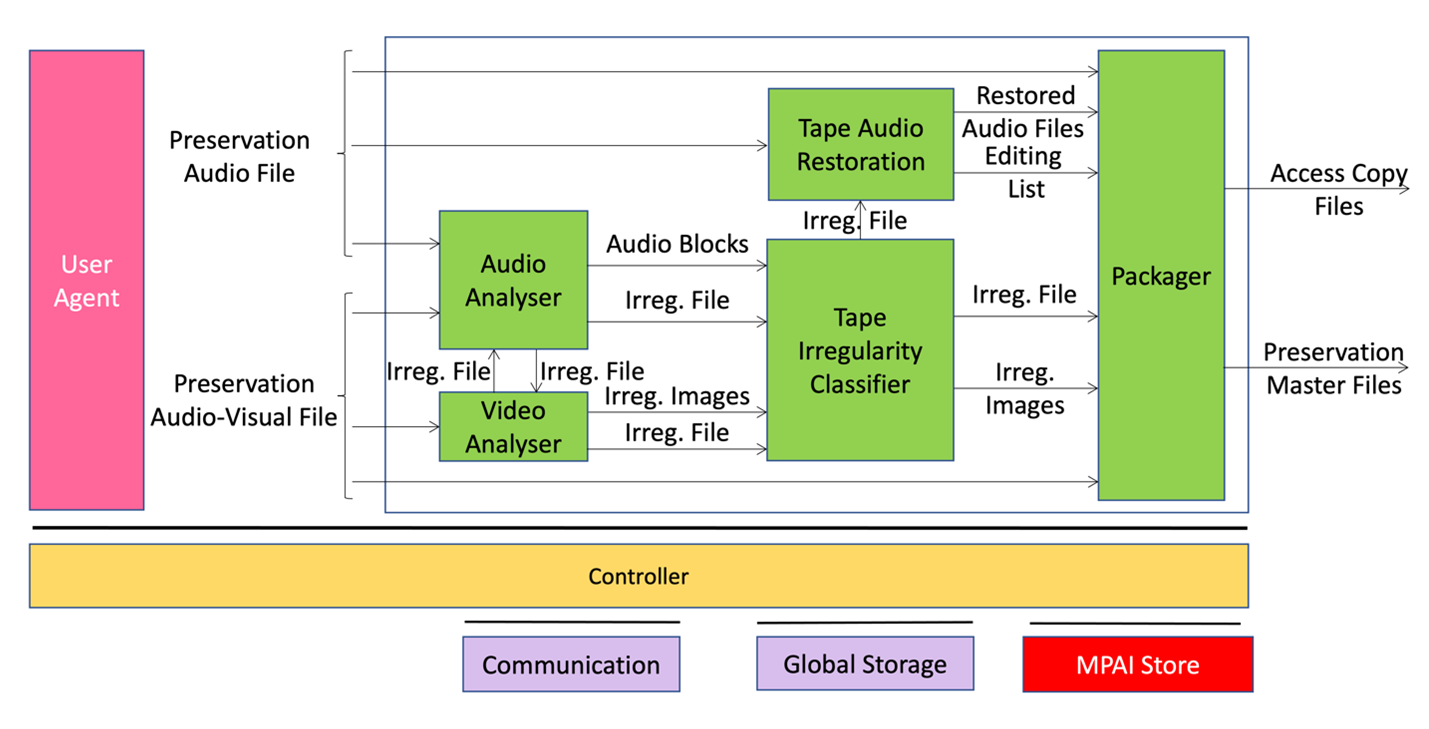
\includegraphics[width=\textwidth]{arp-workflow.png}
    \caption{\ac{AIW} di \acl{ARP}}
    \label{fig:arp-workflow}
\end{figure}

Facendo riferimento alla figura \ref{fig:arp-workflow} gli \acp{AIM} di \ac{ARP} sono:
\begin{description}
    \item[Audio Analyser] È l'\ac{AIM} che rileva le irregolarità nell'audio, estrae i segmenti di \qty{500}{\ms} in loro corrispondenza e li invia al classificatore.
    \item[Video Analyser] È l'\ac{AIM} che rileva le irregolarità nel video e cattura delle immagini in loro corrispondenza.
    \item[Tape Irregularity Classifier] È l'\ac{AIM} che classifica le irregolarità di audio e video a partire dalle irregolarità rilevate da audio analyser e video analyser.   % TODO nel codice è compreso in aa e va? -> chiedere
    \item[Tape Audio Restoration] È l'\ac{AIM} che corregge velocità, equalizzazione e registrazione a rovescio dell'audio.
    \item[Packager] È l'\ac{AIM} che produce Access Copy Files e Preservation Master Files a partire dai file ricevuti dall'output degli altri \acp{AIM}.
\end{description}

Si osserva nella letteratura afferente al \ac{CSC} che la classificazione dei problemi dalla traccia audio ha un'accuratezza del $93,7\%$ (esempio in figura \ref{fig:confusion-matrix-audio-classification}) \cite[min. 35:10]{mpaistandardsMPAIPresentsContextbased2023}, mentre per la classificazione dalle immagini si raggiungono valori $\geq 98,9\%$ (esempio in figura \ref{fig:confusion-matrix-audio-classification}) \cite[fig. 3 e p. 70]{prettoComputingMethodologiesSupporting2018}.

\begin{figure}[h]
    \begin{minipage}{\textwidth}
        \centering
        \begin{subfigure}{0.8\textwidth}
            \centering
            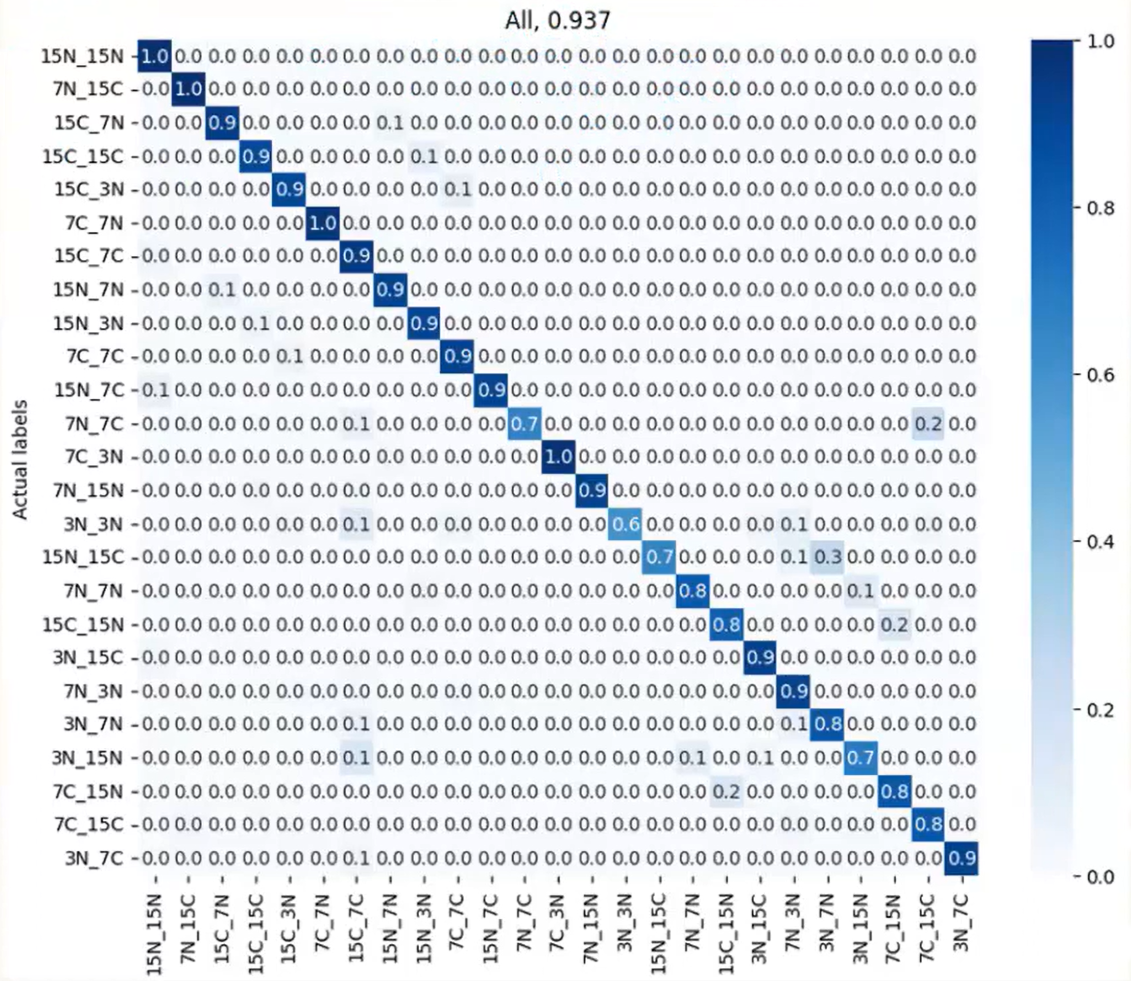
\includegraphics[width=\textwidth]{confusion-matrix-audio-classification.png}
            \caption{Matrice di confusione di classificatore audio \cite[min. 35:10]{mpaistandardsMPAIPresentsContextbased2023}}
            \label{fig:confusion-matrix-audio-classification}
        \end{subfigure}
        \par\bigskip
        \begin{subfigure}{0.9\textwidth}
            \centering
            \begin{subfigure}{0.45\textwidth}
                \centering
                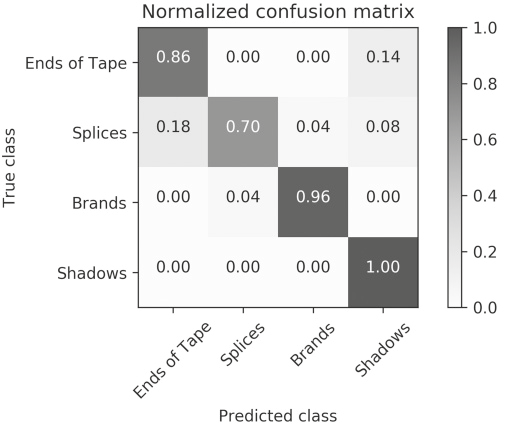
\includegraphics[width=\textwidth]{confusion-matrix-video-classification-7dot5ips-tape.png}
                \caption{Matrice di confusione di classificatore video, esperimento a velocità \qty{7,5}{ips}}
                \label{fig:confusion-matrix-video-classification-7dot5ips-tape}
            \end{subfigure}
            \hfill
            \begin{subfigure}{0.45\textwidth}
                \centering
                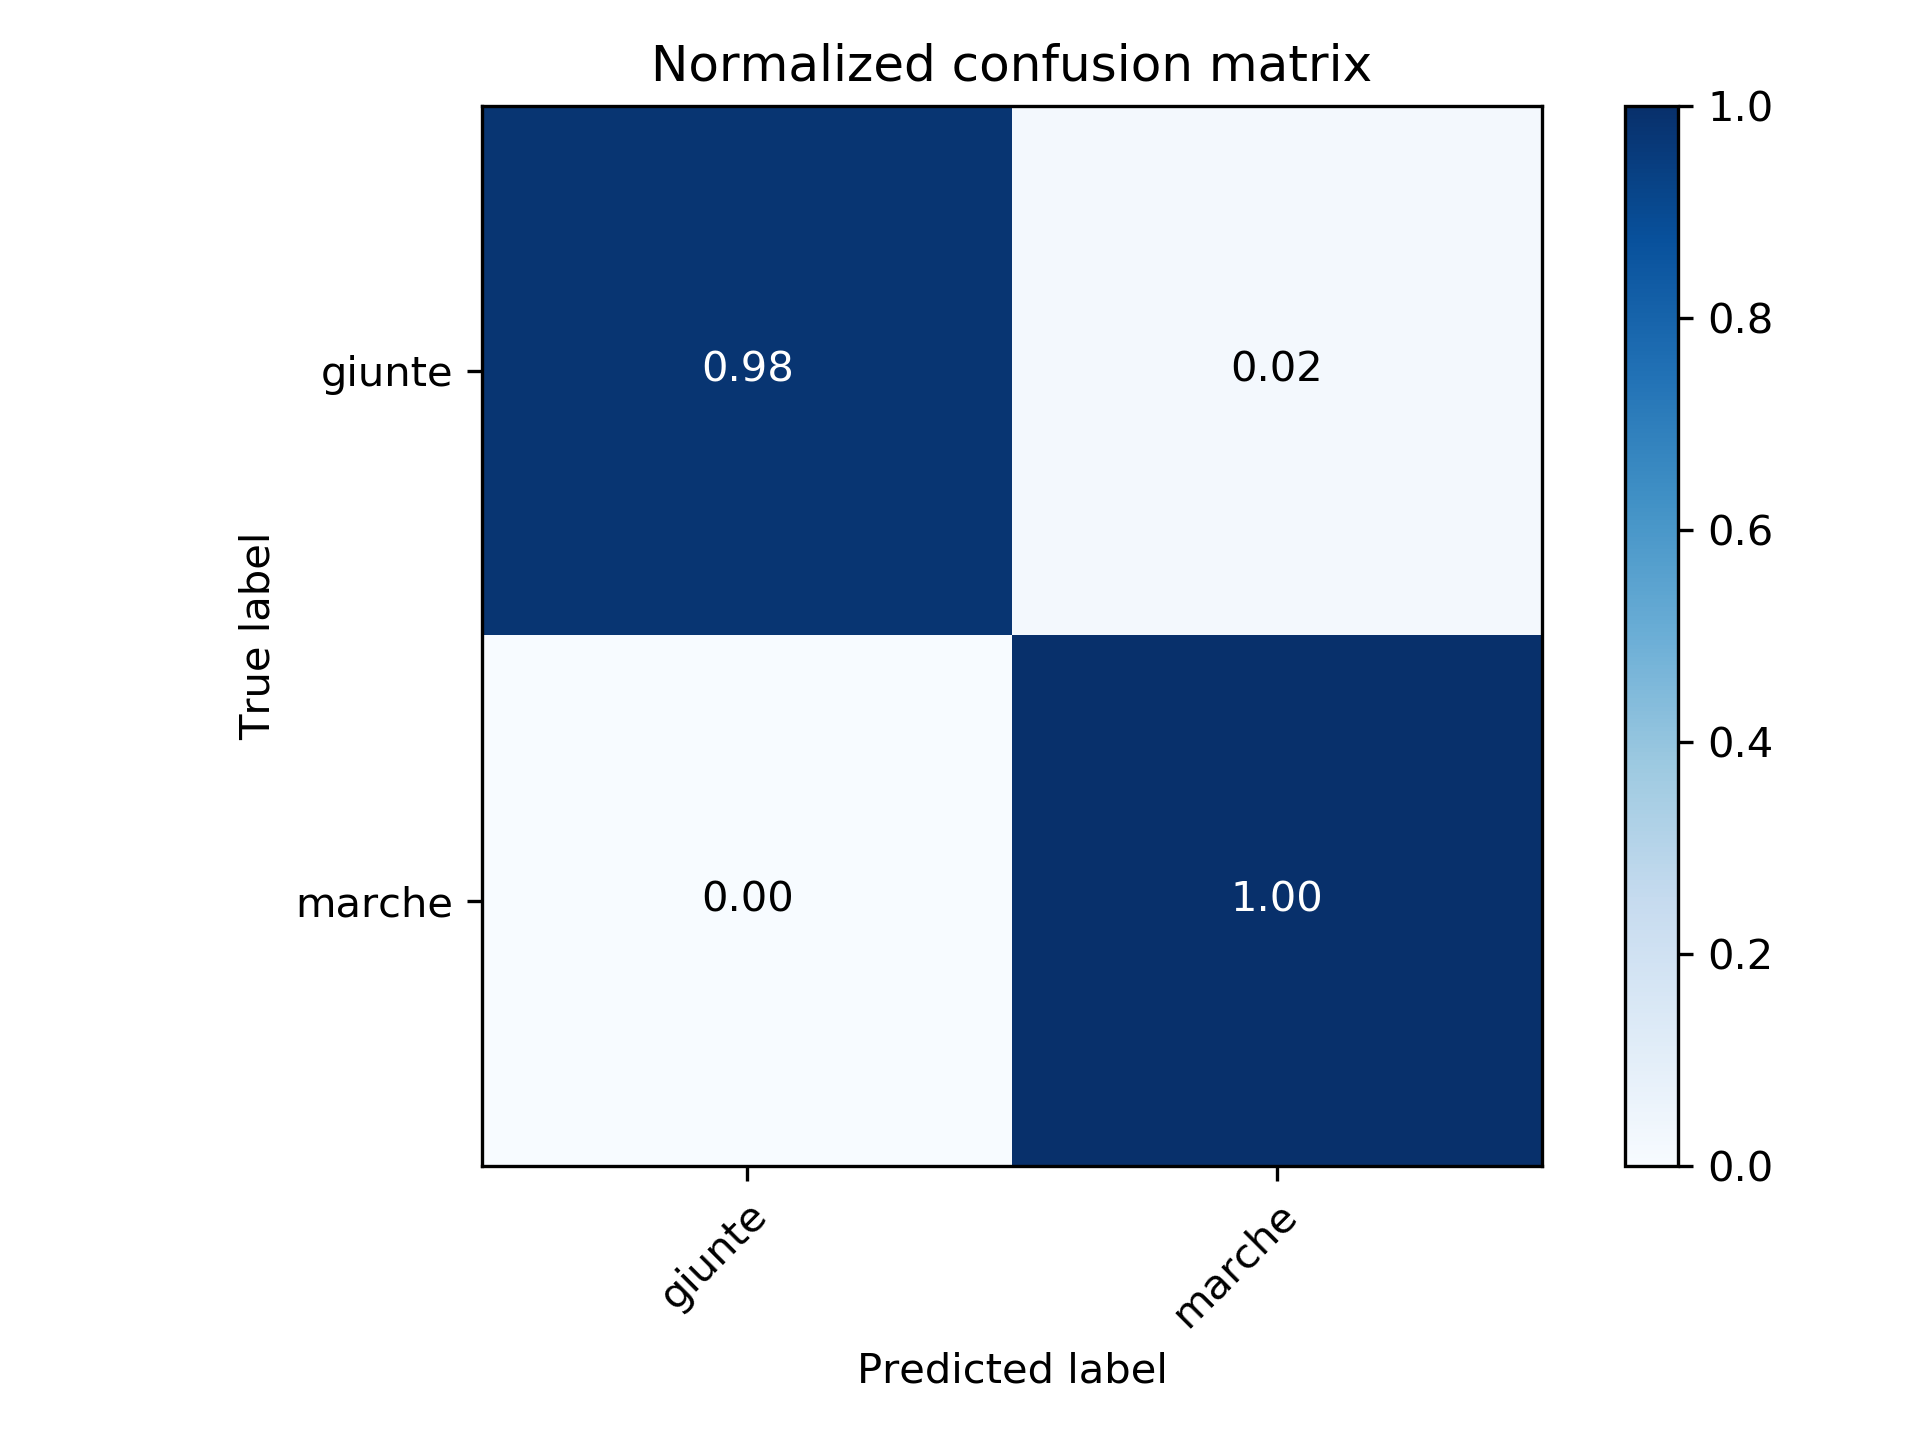
\includegraphics[width=\textwidth]{confusion-matrix-video-classification-15ips-tape.png}
                \caption{Matrice di confusione di classificatore video, esperimento a velocità \qty{15}{ips}}
                \label{fig:confusion-matrix-video-classification-15ips-tape}
            \end{subfigure}
            \caption{Matrice di confusione di classificatore video \cite[fig. 3]{prettoComputingMethodologiesSupporting2018}}
            \label{fig:confusion-matrix-video-classification}
         \end{subfigure}
            \caption[Matrici di confusione da esperimenti in letteratura con classificatori per \ac{ARP}.]{Matrici di confusione\footnotemark da esperimenti in letteratura con classificatori per \ac{ARP}.}
            \label{fig:confusion-matrix-audio-video}
        \mpfootnotes
        \footnotetext{Una matrice di confusione, \textit{confusion matrix} è una rappresentazione visuale dell'accuratezza di un classificatore, ogni colonna rappresenta i valori predetti ed ogni riga i valori reali, in corrispondenza di ogni intersezione si trova il valore assoluto o la percentuale di volte in cui si è verificata tale intersezione.}
    \end{minipage}
\end{figure}

Le tipologie di irregolarità previste e riconosciute dallo standard sono riassunte nella tabella \ref{tab:arp-irrs}.

\begin{table}[h]
    \centering
    \begin{tabular}{|c|c|}
        \hline
        \textbf{Acronym} &      \textbf{Meaning}\\
        \hline
        B       &   Brands on tape\\
        DA      &   Damaged tape\\
        DI      &   Dirt\\
        EOT     &   Ends of tape\\
        ESV     &   Equalization standard variation\\
        M       &   Marks\\
        PPS     &   Play, pause, stop\\
        PSD     &   Power spectral density\\
        RMSE    &   Root Mean Square Error\\
        S       &   Shadows\\
        SB      &   Signal Backward\\
        SOT     &   Start of tape\\
        SP      &   Splice\\
        SSV     &   Speed standard variation\\
        WF      &   Wow and flutter\\
        \hline
    \end{tabular}
    \caption{Irregolarità rilevate da \ac{ARP}} \cite[tab. 21-22]{ieeeStandard3302-2022}
    \label{tab:arp-irrs}
\end{table}


% TODO scrivere di più? o basta quello scritto in csc-digitalizzazione; in caso aggiungere alla fine